

\section{Discriminant Analysis in R}

The function \texttt{lda()}, found in the R library \texttt{MASS}, carries out linear discriminant analysis (i.e. canonical variates analysis). 


\begin{R}
> library(MASS) #load the MASS package
> z <-lda(Species ~ Sepal.Length + Sepal.Width + Petal.Length + Petal.Width,
+           iris, prior=c(1,1,1)/3)
> z
Call:
lda(Species ~ Sepal.Length + Sepal.Width + Petal.Length + Petal.Width, 
    data = iris, prior = c(1, 1, 1)/3)

Prior probabilities of groups:
    setosa versicolor  virginica 
 0.3333333  0.3333333  0.3333333 

Group means:
           Sepal.Length Sepal.Width Petal.Length Petal.Width
setosa            5.006       3.428        1.462       0.246
versicolor        5.936       2.770        4.260       1.326
virginica         6.588       2.974        5.552       2.026

Coefficients of linear discriminants:
                    LD1         LD2
Sepal.Length  0.8293776  0.02410215
Sepal.Width   1.5344731  2.16452123
Petal.Length -2.2012117 -0.93192121
Petal.Width  -2.8104603  2.83918785

Proportion of trace:
   LD1    LD2 
0.9912 0.0088 
\end{R}

The |prior| argument given in the |lda()| function call isn't strictly necessary because by default the |lda| function will assign equal probabilities among the groups. However I included this argument call to illustrate how to change the prior if you wanted. The output give some simple summary statistics for the group means for each of the variables and then gives the coefficients of the canonical variates.  The `Proportion of trace' output above tells us that 99.12\% of the between-group variance is captured along the first discriminant axis.

\subsection{Shorthand Formulae in R}

You've encountered the use of model formulae in R several times, such as in the call to |lda()| above and when carrying out various regressions.  The document ``An Introduction to R" (distributed with R and available at the R project website) gives a concise summary and a number of examples of how to construct formulae in R (see \href{http://cran.r-project.org/doc/manuals/R-intro.html#Formulae-for-statistical-models}{Defining statistical models: formulae}).

Relevant to our current example is a shorthand way for specifying multiple variables in a formula. In the example above we called the |lda()| function with a formula of the form: 
\begin{R}
Species ~ Sepal.Length + Sepal.Width + ....
\end{R}

Writing the names of all those variables is tedious and error prone and would be unmanageable if we were analyzing a data set with tens or hundreds of variables. Luckily we can use the shorthand name `|.|' to specify all other variables in the data frame except the variable on the left.  For example, we can rewrite the |lda()| call above as:

\begin{R}
> z <- lda(Species ~ ., data = iris, prior = c(1,1,1)/3)
\end{R}

\subsection{Fine Tuning Your Plot}

To get a graphical representation of the specimens in the space of the canonical variates you can use the |plot()| function on the object returned by the call to |lda()|.

\begin{R}
> plot(z) # 2D scatter plot of specimens in CVs 1 and 2
> plot(z, abbrev=T) # use abbreviated group names
\end{R}

You can also create a plot to look at group variation along just the first canonical variate:

\begin{R}
> plot(z, dimen=1,type='both') # plot histograms and density plots for each group along 1st CV 
\end{R}


The plot call on the object returned by |lda()| allows some additional customization of the plot, but the extent of graphical tuning is limited:

\begin{R}
> plot(z, abbrev=T, xlab='CV1', ylab='CV2') # change the x- and y- labels
\end{R}

If you want to do any more fine tuning of the plot you'll have to calculate the CV scores from the coefficients and reconstruct the plot to your liking. Below I give an example of how to do that:

\begin{R}
> iris.data <- subset(iris,select=-Species)
> iris.mtx <- as.matrix(iris.data)
> dim(iris.mtx)
[1] 150   4
> iris.cv <- iris.mtx %*% z$scaling # gives scores in the CV space
> dim(iris.cv)
[1] 150   2
> group.symbols <- (1:3)[iris$Species] # specify the symbols for each group
> plot(iris.cv, pch=group.symbols, asp=1, xlab="CV1", ylab="CV2")
\end{R}

The definition of |group.symbols| and the use of the |pch| argument require a little explanation. |pch| is short-hand for `plotting  character' and specifies the symbols used to represent each observation in the plot.  These symbols can either be letters or integers in the range 0-25. The integers refer to a standard set of symbols shapes defined in R. Figure~1 gives those symbols.

\begin{figure}
\begin{center}

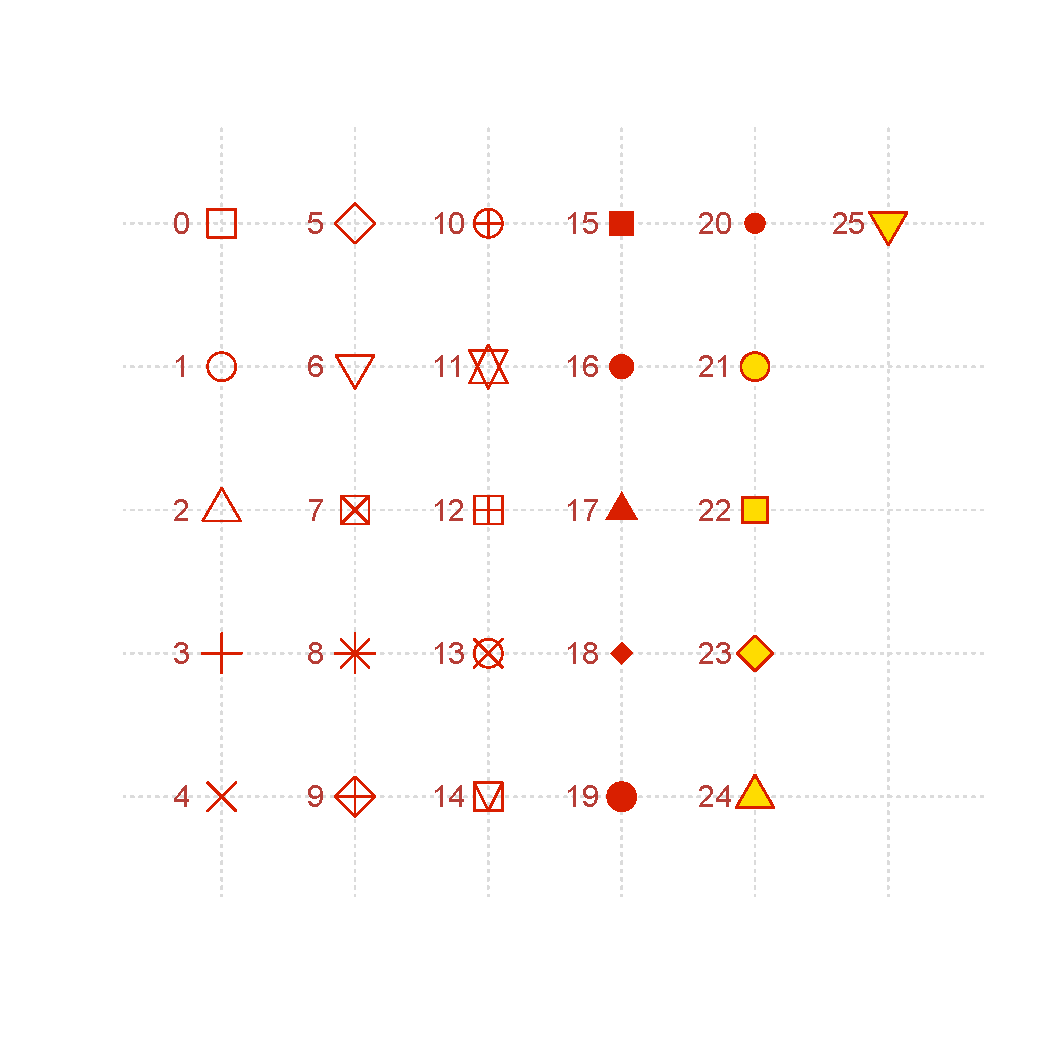
\includegraphics[width=0.5\columnwidth]{./figures/hands-on8/pch-symbols}

\end{center}
\caption{Standard R symbols, and their corresponding integer values, accessible via the \texttt{pch} argument to plot.}
\end{figure}

If you'd like to see a function that prints out all the standard symbols type |?points| and check out the |pchShow| function defined in the example at the bottom of the documentation page.  To see this example in action type |example(points)|. After typing |example(points)| you can call the |pchShow| function directly (that's how I generated the figure).

The |group.symbols <- ...| line constructs a vector of length $n$ (where $n$ is the length of the \lstinline|iris$Species| vector) where each element of the |group.symbols| vector has the value 1, 2 or 3 according to which species the corresponding specimen represents.  A simpler example might make this clearer:

\begin{R}
> sexes = as.factor(c('M','F','F','M','F'))
> sexes
[1] M F F M F
Levels: F M
> c("a","b")[sexes]
[1] "b" "a" "a" "b" "a"
\end{R}

Here I created a simple example involving five specimens where each specimens was categorized by sex. The |as.factor| function tells R to treat the characters in the vector as factor levels. I then assigned each specimen a label, either``a" or ``b" depending on its sex.  If I wanted to extend that example to our three species iris data set I could do something like:

\begin{R}
> group.symbols = c("a","b","c")[iris$Species]
> plot(iris.cv, pch=group.symbols, cex=0.75, asp=1, xlab="CV1", ylab="CV2")
\end{R}

This draws each specimen with the label ``a", ``b", or ``c" depending on which species it is assigned to. Notice that in the last example I used the |cex| argument to make the symbols smaller than normal.  

What if i wanted to also plot the group means in the canonical variate space?  The following example shows how to do that:

\begin{R}
> group.symbols = c(0,2,4)[iris$Species] # I switched back to symbols 
> group.colors = c('red','darkorange','blue')[iris$Species] # I also want to use colors 
> cv1.means <- tapply(iris.cv[,1], iris$Species, mean)
> cv1.means
    setosa versicolor  virginica 
  5.502493  -3.930156  -7.887657 
> cv2.means <- tapply(iris.cv[,2], iris$Species, mean)
> cv2.means
    setosa versicolor  virginica 
  6.876606   5.933573   7.174239 
> plot(iris.cv, pch=group.symbols, cex=0.75, asp=1, 
+       xlab="CV1", ylab="CV2", col=group.colors)
> points(cv1.means, cv2.means, pch=16, cex=1.5, col='black')
\end{R}

Note the use of the |points()| function. This function draws on top of rather than erasing the previous plot.  Note too the use of the |col| argument in the |plot()| call to specify different colors.  If you'd like to see a chart of all the colors in R check out this web page: \href{http://research.stowers-institute.org/efg/R/Color/Chart/}{A Chart of R Colors}.

I stated in lecture that for the canonical variate diagram we can estimate the $100(1-\alpha)$ confidence region for a group mean as a circle centered at the mean having a radius $(\chi^{2}_{\alpha,r}/n_i)^{1/2}$ where $r$ is the number of canonical variate dimensions considered. Using similar reasoning the $100(1-\alpha)$ confidence region for the whole population is given by a hypersphere centered at the mean with radius $(\chi^{2}_{\alpha,r})^{1/2}$.  
To calculate these confidence regions you could look up the appropriate value of the the  $\chi^2$ distribution in a book of statistical tables, or we can use the |qchisq()| function which gives the inverse cumulative probability distribution for the $\chi^2$ function:

\begin{R}
> chi2 = qchisq(0.05,2, lower.tail=F)
> chi2
[1] 5.991465
> group.lengths = tapply(iris$Species, iris$Species, length)
> group.lengths
    setosa versicolor  virginica 
        50         50         50 
> mean.radii = sqrt(chi2/group.lengths)
> pop.radii = rep(sqrt(chi2),3)
> help.search("circle")  # I don't remember off hand how to draw circles so let's look it up
> library(tripack) # Let's use the circles function in the 'tripack' package
> circles(cv1.means, cv2.means, pop.radii,lty='dashed') 
> circles(cv1.means, cv2.means, mean.radii,lty='dotted')
\end{R}

Let's put the finishing touch on our plots by adding some color coded rug plots to the first CV axis. For completeness I'll include all the previous steps used to generate the plot:

\begin{R}
> plot(iris.cv, pch=group.symbols, cex = 0.75, asp=1, xlab="CV1", ylab="CV2", col=group.colors)
> points(cv1.means, cv2.means, pch=16, cex=1.5,col='red')
> circles(cv1.means, cv2.means, pop.radii,lty='dashed')
> circles(cv1.means, cv2.means, mean.radii, lty='dotted')
> rug(iris.cv[,1][iris$Species=="setosa"],col="red")
> rug(iris.cv[,1][iris$Species=="versicolor"],col="darkorange")
> rug(iris.cv[,1][iris$Species=="virginica"],col="blue")
> title("Canonical Variates Analysis\nof Anderson's Iris Data")
\end{R}


If you did everything right (and I cut and pasted correctly!) you should get a plot that looks like \cref{fig:cva}.

\begin{figure}
\begin{center}
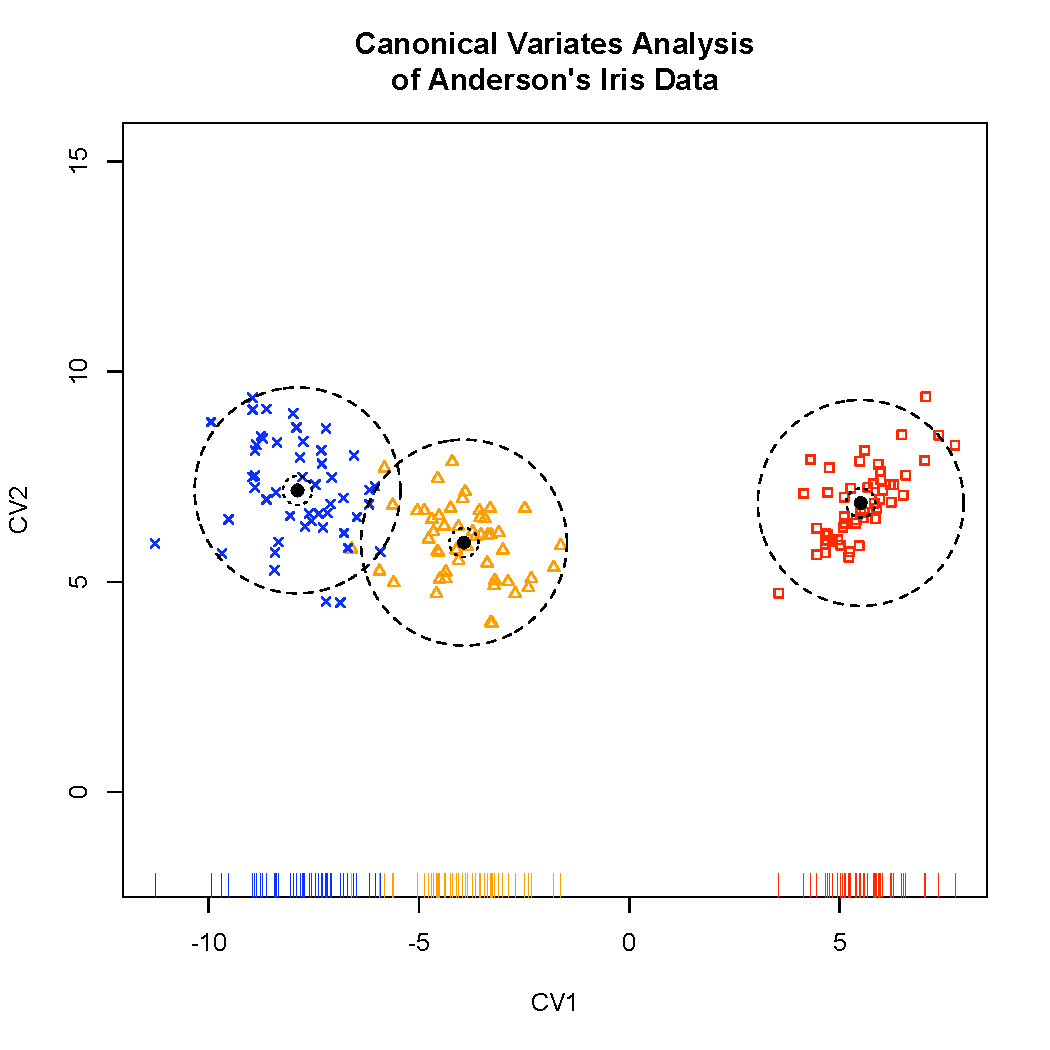
\includegraphics[height=0.5\columnwidth]{./figures/hands-on8/iris-cva-fancy}
\end{center}
\caption{Ordination of iris specimens in the space of the first two canonical variates.  The dashed circles surrounding each species distribution give the approximate 95\% tolerance regions for the population distributions. See text for details on the construction of this plot.} \label{fig:cva}.
\end{figure} If I was going to be repeatedly generate these types of plots I would wrap up the key steps discussed above into a convenient function.


\subsection{Calculating the Within and Between Group Covariance Matrices}

The |lda()| function conveniently carries out the key steps of a canonical variates analysis for you.  However, what if we wanted some of the intermediate matrices relevant to the analysis such as the within- and between group covariances matrices? The code below shows you how to calculate these:

\begin{R}
> g = iris$Species
> group.means <- rowsum(iris.mtx, g)/as.vector(table(g))
> group.means
           Sepal.Length Sepal.Width Petal.Length Petal.Width
setosa            5.006       3.428        1.462       0.246
versicolor        5.936       2.770        4.260       1.326
virginica         6.588       2.974        5.552       2.026
> Dwin <- iris.mtx - group.means[g,]
> nobs <- dim(iris.mtx)[1]
> ngroups <- length(levels(g))
> win.cov <- 1/(nobs-ngroups) * t(Dwin) %*% Dwin
> btw.cov.unweighted <- cov(group.means)
\end{R}

Having now calculated the within group covariance matrix we can calculate the Mahalanobis distance between the means of each group as follows:

\begin{R}
> mahalanobis(group.means, group.means[1,], win.cov)
    setosa versicolor  virginica 
   0.00000   89.86419  179.38471 
> mahalanobis(group.means, group.means[2,], win.cov)
    setosa versicolor  virginica 
  89.86419    0.00000   17.20107 
> mahalanobis(group.means, group.means[3,], win.cov)
    setosa versicolor  virginica 
 179.38471   17.20107    0.00000 
\end{R}

\medskip
\begin{assignment}
\small

Identify a paper from the literature (published in the last decade) that employs one or more of the following multivariate statistical techniques:

\begin{enumerate}
\item Multivariate regression
\item Principal Component Analysis
\item Singular Value Decomposition
\item Canonical Variate Analysis (or an alternate discriminant function)
\end{enumerate}

Write a short report discussing the use of these techniques in the paper and how the application of these methods contributed to the author's conclusions or understanding of the data.  Your report should touch on any assumptions (explicit or implicit) that are relevant to the statistical analysis and discuss whether you feel the author's conclusions are justified or well supported (again based on the statistical anlaysis).

\medskip
Include in your report a brief outline (bullet points) that lays out the key steps (e.g. handling of missing data, normalization) and the primary R functions that you would use to repeat the analysis yourself. Specify whether the author(s) have made their multivariate data set available.


\end{assignment}


